\documentclass[conference]{IEEEtran}

% ---- Fonts & math (LuaLaTeX対応) ----
\usepackage{newtxtext,newtxmath}

% ---- Graphics & color ----
\usepackage{graphicx}
\usepackage[dvipsnames]{xcolor}

% ---- Spacing around floats (tight for 2 pages) ----
\setlength{\textfloatsep}{5pt plus 1pt minus 1pt}
\setlength{\floatsep}{5pt plus 1pt minus 1pt}
\setlength{\intextsep}{5pt plus 1pt minus 1pt}

% ---- Tables ----
\usepackage{booktabs}

% ---- Float control ----
\usepackage{placeins}

% ---- TikZ ----
\usepackage{tikz}
\usetikzlibrary{
  arrows.meta,
  positioning,
  fit,
  calc,
  shapes.geometric,
  shapes.misc
}

% ---- TikZ styles (NOTE: step -> flowstep to avoid key clash) ----
\tikzset{
  line/.style={-Latex, line width=0.45pt},
  box/.style={draw, rounded corners=2pt, align=center, inner sep=3pt, minimum height=7.2mm},
  smallbox/.style={box, minimum width=26mm},
  midbox/.style={box, minimum width=32mm},
  bigbox/.style={box, minimum width=64mm},
  flowstep/.style={box, minimum width=30mm} % <— was 32mm; a bit tighter
}

% ---- Convenience ----
\newcommand{\etal}{\textit{et~al.}}

% =========================================================
\begin{document}

\title{AITL on Space: A Robust Three-Layer Architecture\\
with a Tri-NVM Hierarchy (SRAM / MRAM / FRAM)\\
for Long-Duration Spacecraft Autonomy}

\author{\IEEEauthorblockN{Shinichi Samizo}\\
\IEEEauthorblockA{Independent Semiconductor Researcher\\
Former Engineer at Seiko Epson Corporation\\
Email: shin3t72@gmail.com\quad GitHub: \url{https://github.com/Samizo-AITL}}
}

\maketitle

\begin{abstract}
\noindent
We propose \textit{AITL on Space}, a robust three-layer control architecture (Robust Core, FSM Supervisor, AI Adaptor) integrated with a tri-NVM hierarchy (SRAM/MRAM/FRAM) and mapped to a 22\,nm FDSOI SoC. The contribution is a complete end-to-end design flow from mission-level specification to ASIC: requirements are formalized as JSON via EduController, synthesized by the AITL-H module, validated in FPGA HIL with fault injection, stress-tested through SystemDK FEM (thermal/radiation/packaging), and finally implemented as ASIC. This methodology enables resilient autonomy for long-duration spacecraft missions.
\end{abstract}

\section{Introduction}
Deep-space missions require ultra-robust control under total ionizing dose (TID), single event effects (SEE), and thermal cycling. Conventional PID\,+\,Flash architectures face lifetime limits due to charge-trap drift and endurance. We present \emph{AITL on Space}: a resilient three-layer architecture with a tri-NVM hierarchy and a reproducible design flow from specification to ASIC.

\section{Specification and Design Flow}
The process begins with \textbf{Mission Specification}. Requirements such as pointing accuracy, power stability, and thermal tolerance are captured in \textbf{EduController}, a model-based tool that exports plant matrices and weighting functions as JSON (portable across simulators). The JSON is consumed by \textbf{AITL-H}, which synthesizes an $H_\infty$ output-feedback controller $K$ with mixed-sensitivity weighting and generates a fixed-point implementation for RTL/FPGA/ASIC. The design then undergoes:
\begin{itemize}[itemsep=0pt,topsep=1pt,leftmargin=*]
  \item \textbf{FPGA HIL}: hardware-in-the-loop validation with SEU\,+\,outage injection; metrics include safe-mode entry $<\!1$\,s, recovery rate $\ge 99\%$, and ECC scrubbing efficiency.
  \item \textbf{SystemDK FEM}: co-simulation of thermal cycles, radiation effects, and packaging stress, closing the verification loop before silicon.
  \item \textbf{ASIC Mapping}: implementation on GlobalFoundries 22FDX FDSOI hardened for long-duration missions.
\end{itemize}
\textit{Toolchain at a Glance}. \emph{EduController} $\rightarrow$ spec\,$\rightarrow$\,JSON exporter (plant $A,B,C,D$, noise/disturbance models, weights $W_1,W_2,W_3$). \emph{AITL-H}: $H_\infty$ synthesizer (Riccati/LMI)\,$\rightarrow$\,fixed-point $K$. \emph{SystemDK FEM} = thermal/radiation/packaging derating \& memory scrubbing validation.

\section{System Architecture}
AITL consists of three layers:
\begin{itemize}[itemsep=0pt,topsep=1pt,leftmargin=*]
  \item \textbf{Robust Core}: $H_\infty$/MPC/SMC controllers for stability.
  \item \textbf{FSM Supervisor}: mode switching (Safe/Nominal/Recovery) with FDI/FDI\!I for fault management.
  \item \textbf{AI Adaptor}: long-term re-identification and drift compensation.
\end{itemize}
A tri-NVM hierarchy ensures persistence: SRAM for execution, MRAM for logs/code with ECC scrubbing and dual slots, and FRAM for safe boot and FSM states. Target SoC is 22\,nm FDSOI hardened for radiation and temperature stress.

\section{Mathematical Model and $H_\infty$ Design}
We consider an 11D discrete-time state-space plant coupling attitude (6), power bus (2), and thermal nodes (3):
\begin{align}
x_{k+1} &= A x_k + B u_k + E w_k,\\
y_k     &= C x_k + D u_k + v_k,
\end{align}
where $w_k$ and $v_k$ are disturbance and noise. The model extends to 20D by adding translational axes and bias states. Weights $(W_1,W_2,W_3)$ shape sensitivity, control effort, and complementary sensitivity. \textit{EduController} outputs them as JSON; \textit{AITL-H} synthesizes $K$ with robustness margins and exports a fixed-point realization for RTL/FPGA/ASIC.

\section{Verification Pipeline}
FPGA HIL injects SEUs and sensor outages. Metrics include safe-mode entry time ($<\!1$\,s), recovery rate ($\ge 99\%$), and ECC scrubbing efficiency. \textit{SystemDK FEM} validates thermal and radiation stress, ensuring packaging reliability before ASIC tape-out.

\section{Conclusion}
\textit{AITL on Space} combines robust control, supervisory safety, AI re-identification, and hardened memory. The proposed end-to-end flow—from mission specification to ASIC—provides a reproducible methodology for resilient autonomy in long-duration space missions.

% Balance last page columns around ref. 3 (tune as needed)
\IEEEtriggeratref{3}

\begin{thebibliography}{4}
\bibitem{doyle} J.~C. Doyle, B.~A. Francis, and A.~R. Tannenbaum, \emph{Feedback Control Theory}. Macmillan, 1992.
\bibitem{colinge} J.-P. Colinge, \emph{Silicon-on-Insulator Technology: Materials to VLSI}, 3rd ed. Springer, 2004.
\bibitem{wolf} W. Wolf, \emph{FPGA-Based System Design}. Prentice Hall, 2004.
\bibitem{rabey} J.~M. Rabaey, A. Chandrakasan, and B. Nikolić, \emph{Digital Integrated Circuits: A Design Perspective}, 2nd ed. Prentice Hall, 2003.
\end{thebibliography}

\section*{Author Biography}
\begingroup\small
Shinichi Samizo received the M.S. degree in Electrical and Electronic Engineering from Shinshu University, Japan. He worked at Seiko Epson Corporation as an engineer in semiconductor memory and mixed-signal device development, and contributed to inkjet MEMS actuators and PrecisionCore printhead technology. He is currently an independent semiconductor researcher focusing on process/device education, memory architecture, and AI system integration. Contact: \texttt{shin3t72@gmail.com}.
\endgroup

% =========================================================
% Figures (AFTER biography). Fig.1 & Fig.3 are single-column, Fig.2 is double.

\FloatBarrier

% -------- Fig.1: End-to-end flow (single column, bottom) --------
\begin{figure}[!b]
\centering
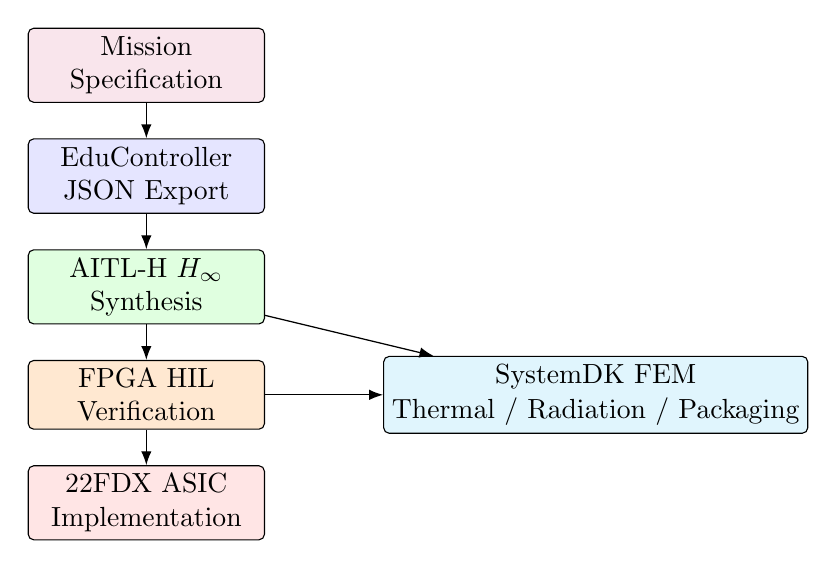
\begin{tikzpicture}[node distance=4.5mm]
  \node[flowstep, fill=purple!10]                 (spec) {Mission\\Specification};
  \node[flowstep, fill=blue!10,   below=of spec]  (json) {EduController\\JSON Export};
  \node[flowstep, fill=green!12,  below=of json]  (hinf) {AITL-H $H_\infty$\\Synthesis};
  \node[flowstep, fill=orange!18, below=of hinf]  (hil)  {FPGA HIL\\Verification};
  \node[flowstep, fill=red!10,    below=of hil]   (asic) {22FDX ASIC\\Implementation};
  \node[flowstep, fill=cyan!12,   right=15mm of hil] (fem) {\shortstack{SystemDK FEM\\Thermal / Radiation / Packaging}};

  \draw[line] (spec) -- (json);
  \draw[line] (json) -- (hinf);
  \draw[line] (hinf) -- (hil);
  \draw[line] (hil)  -- (asic);
  \draw[line] (hinf) -- (fem);
  \draw[line] (hil)  -- (fem);
\end{tikzpicture}
\caption{End-to-end design flow: Mission Spec $\rightarrow$ JSON (EduController) $\rightarrow$ AITL-H $\rightarrow$ FPGA HIL $\rightarrow$ FEM $\rightarrow$ ASIC.}
\label{fig:flow}
\end{figure}

% -------- Fig.2: Architecture with tri-NVM (double column, top) --------
\begin{figure*}[!t]
\centering
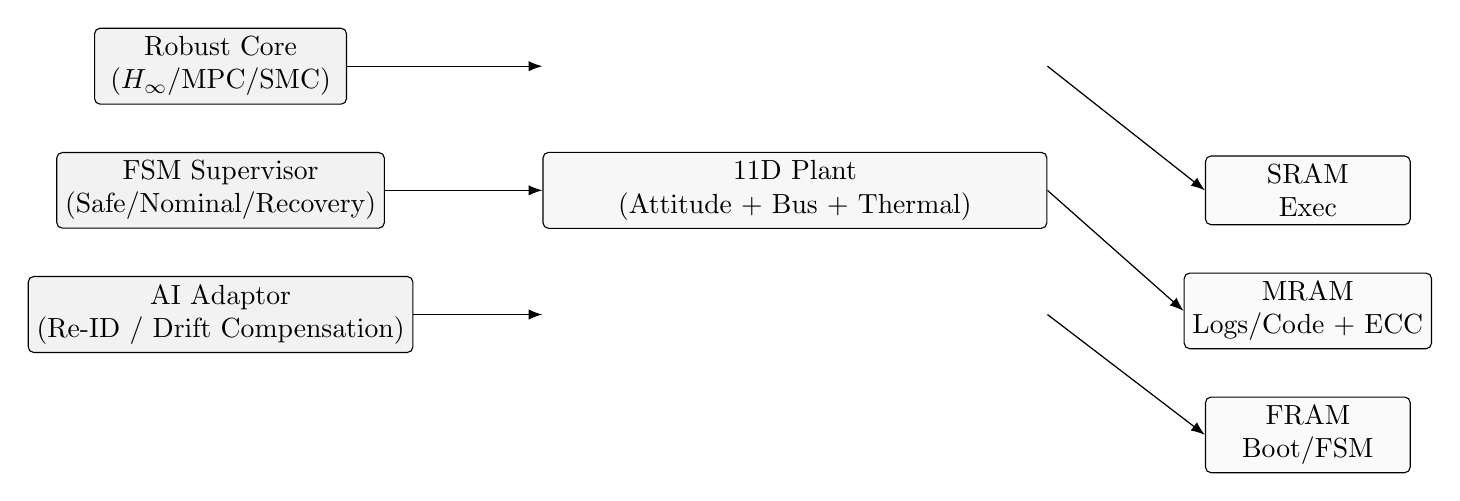
\begin{tikzpicture}[node distance=6mm]
  % Left: three control layers
  \node[midbox, fill=black!5] (robust) {Robust Core\\($H_\infty$/MPC/SMC)};
  \node[midbox, fill=black!5, below=of robust] (fsm) {FSM Supervisor\\(Safe/Nominal/Recovery)};
  \node[midbox, fill=black!5, below=of fsm] (ai) {AI Adaptor\\(Re-ID / Drift Compensation)};

  % Plant block
  \node[bigbox, fill=black!3, right=20mm of fsm] (plant) {11D Plant\\(Attitude + Bus + Thermal)};

  % NVM hierarchy to the right
  \node[smallbox, fill=black!2, right=20mm of plant] (sram) {SRAM\\Exec};
  \node[smallbox, fill=black!2, below=of sram] (mram) {MRAM\\Logs/Code + ECC};
  \node[smallbox, fill=black!2, below=of mram] (fram) {FRAM\\Boot/FSM};

  % Connections
  \draw[line] (robust) -- (plant.west |- robust);
  \draw[line] (fsm)    -- (plant.west |- fsm);
  \draw[line] (ai)     -- (plant.west |- ai);

  \draw[line] (plant.east |- robust) -- (sram.west);
  \draw[line] (plant.east |- fsm)    -- (mram.west);
  \draw[line] (plant.east |- ai)     -- (fram.west);
\end{tikzpicture}

\medskip
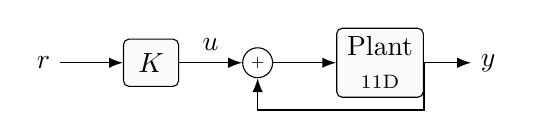
\begin{tikzpicture}[node distance=6mm]
  % Closed-loop schematic (compact)
  \node[box, minimum width=7mm, minimum height=6mm, fill=black!2] (K) {$K$};
  \node[circle, draw, inner sep=0pt, minimum size=3.8mm, right=8mm of K] (sum) {\tiny$+$};
  \node[box, minimum width=11mm, minimum height=6mm, fill=black!2, right=8mm of sum] (P) {Plant\\\scriptsize 11D};

  \node[left=8mm of K] (r) {$r$};
  \node[right=6mm of P] (y) {$y$};

  \draw[line] (r) -- (K);
  \draw[line] (K) -- node[above, yshift=0.3mm] {$u$} (sum);
  \draw[line] (sum) -- (P);
  \draw[line] (P) -- (y);
  \draw[line] (P.east) |- ++(0,-6mm) -| (sum.south); % feedback
\end{tikzpicture}
\caption{(Top) AITL architecture: three control layers with tri-NVM memory hierarchy. Orthogonal interconnects improve readability. (Bottom) Closed-loop for $H_\infty$ mixed-sensitivity synthesis on the 11D plant.}
\label{fig:arch}
\end{figure*}

% -------- Fig.3: Small closed-loop (single column, bottom) --------
\begin{figure}[!b]
\centering
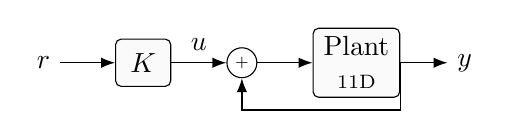
\begin{tikzpicture}[node distance=8mm]
  \node[box, minimum width=7mm, minimum height=6mm, fill=black!2] (K) {$K$};
  \node[circle, draw, inner sep=0pt, minimum size=3.8mm, right=7mm of K] (sum) {\tiny$+$};
  \node[box, minimum width=11mm, minimum height=6mm, fill=black!2, right=7mm of sum] (P) {Plant\\\scriptsize 11D};
  \node[left=7mm of K] (r) {$r$};
  \node[right=6mm of P] (y) {$y$};
  \draw[line] (r) -- (K);
  \draw[line] (K) -- node[above, yshift=0.3mm] {$u$} (sum);
  \draw[line] (sum) -- (P);
  \draw[line] (P) -- (y);
  \draw[line] (P.east) |- ++(0,-6mm) -| (sum.south);
\end{tikzpicture}
\caption{Closed-loop system for $H_\infty$ synthesis (compact single-column rendering).}
\label{fig:loop}
\end{figure}

\end{document}
